\documentclass[dsc,numbers]{coppe}
\usepackage[utf8]{inputenc}
\usepackage{amsmath,amssymb}
\usepackage{hyperref}
\usepackage{siunitx}
\usepackage{booktabs}
\usepackage{cleveref}
\usepackage{minted}

%manter figuras nas seções
\usepackage[section]{placeins}
\makeatletter
\AtBeginDocument{%
	\expandafter\renewcommand\expandafter\subsection\expandafter{%
		\expandafter\@fb@secFB\subsection
	}%
}
\makeatother

%para utilizar subfigures
\usepackage{graphicx}
\usepackage{caption}
\usepackage{subcaption}

%tikz
\usepackage{tikz}
\usetikzlibrary{shapes,arrows}

%localização das figuras
\graphicspath{{IMGS/}}

\makelosymbols
\makeloabbreviations

\begin{document}
  \title{Trabalho - Identificação de Sistemas}
  \foreigntitle{Thesis Title}
  \author{Raphael Timbó}{Silva}
  \advisor{Prof.}{Daniel}{Castello}
  
  \department{PEM}
  \date{01}{2017}

  \keyword{Primeira palavra-chave}
  \keyword{Segunda palavra-chave}
  \keyword{Terceira palavra-chave}

  \maketitle

%  \frontmatter
%  \include{dedic}
%  \include{thanks}
%  \include{resumo}
%  \include{abstract}
  \tableofcontents
  \listoffigures
  \listoftables
  \printlosymbols
  \printloabbreviations


  \mainmatter
  \chapter{Introdução}

O presente trabalho tem por objetivo apresentar os resultados e conclusões referentes ao projeto final da disciplina Identificação de Sistemas.

O trabalho consiste na análise de um sistema através do projeto de um filtro adaptativo FIR. O sistema utilizado é mostrado na \cref{fig:sistema}. 

\begin{figure}[!h]
	\centering
	\includegraphics[width=0.8\textwidth]{IMGS/sistema.pdf}
	\caption{Sistema utilizado na análise.}
	\label{fig:sistema}
\end{figure}

\begin{minted}{python}
class A():
	def __init__(self):
		pass
\end{minted}

Do mesmo modo, é imprescindível definir os símbolos, tal como o
conjunto dos números reais $\mathbb{R}$ e o conjunto vazio $\emptyset$.
\symbl{$\mathbb{R}$}{Conjunto dos n\'umeros reais} empty 
\symbl{$\emptyset$}{Conjunto vazio}		


\section{test}
\subsection{teste}
  \chapter{Dados Pseudo-Experimentais}

\section{Resposta do sistema no tempo} \label{Resposta do sistema no tempo}

Para a construção dos dados pseudo-experimentais foram observados os seguintes casos:

Forçamento:
\begin{itemize}
	\item $F_0(t) = A_0 sin(2\pi f_0 t)$ 
	(Considere $\frac{\omega_1}{2\pi} \leq f_0 \leq \frac{\omega_2}{2\pi})$ 
	\item $F_1(t) = A_1 sin(2\pi f_1 t) + A_2 sin(2\pi f_2 t)$ 
	(Escolha 
	$\frac{0.8 \omega_1}{2\pi} \leq f_j \leq \frac{1.2 \omega_2}{2\pi}$ 
	e
	$A_2 = 2A_1$
	;
	$ j = 1, 2)$
	\item $F_2(t) = $ ruído branco
\end{itemize}

Número de amostras $N$:
\begin{itemize}
	\item $N = 1000$
	\item $N = 5000$
\end{itemize}

Valores para a relação entre sinal e ruído - \abbrev{SNR}{Signal to Noise Ratio} SNR (Signal to Noise Ratio):
\begin{itemize}
	\item $SNR = 90$
	\item $SNR = 50$
	\item $SNR = 10$
\end{itemize}

A \cref{fig:FRF_i2_o2_freq34} mostra a posição da frequência de excitação para a aplicação da força $F_0$, em que uma amplitude $A_0 = 1$ foi utilizada.

\begin{figure}
	\centering
	\includegraphics[scale=1]{FRF_i2_o2_freq34.pdf}
	\caption{Frequência de excitação para a força $F_0$.}
	\label{fig:FRF_i2_o2_freq34}
\end{figure}

A \cref{fig:F0_1000_tempo} mostra a resposta no tempo do sistema ao aplicarmos a força $F_0$ na frequência mostrada na \cref{fig:FRF_i2_o2_freq34} para uma amostragem $N = 1000$. Podemos observar que, para $N=1000$, temos uma excitação de aproximadamente 16 segundos e ainda temos algum transiente na resposta no tempo. Também é possível observar que essa parcela apresenta mais que uma frequência de oscilação.

\begin{figure}
	\centering
	\includegraphics[scale=0.6]{F0_1000_tempo.pdf}
	\caption{Resposta no tempo para a força $F_0$ com $N=1000$.}
	\label{fig:F0_1000_tempo}
\end{figure}

A \cref{fig:F0_5000_tempo} mostra a resposta no tempo para $N=5000$. Neste caso, o tempo vai até aproximadamente 80 segundos e podemos observar que a parcela transiente é praticamente inexistente após os 20 segundos de excitação. Após esse tempo, é esperado que o sistema oscile apenas na frequência de excitação.

\begin{figure}
	\centering
	\includegraphics[scale=0.6]{F0_5000_tempo.pdf}
	\caption{Resposta no tempo para a força $F_0$ com $N=5000$.}
	\label{fig:F0_5000_tempo}
\end{figure}

Para a força $F_1$ a \cref{fig:FRF_i2_o2_freq_1_2} mostra as frequências de excitação que foram aplicadas na massa $m_2$. Podemos notar que nesse caso as forças aplicadas estão próximas as frequências naturais do sistema.

\begin{figure}
	\centering
	\includegraphics[scale=1]{FRF_i2_o2_freq_1_2.pdf}
	\caption{Frequência de excitação para a força $F_1$.}
	\label{fig:FRF_i2_o2_freq_1_2}
\end{figure}

A \cref{fig:F1_5000_tempo} mostra a resposta no tempo para $F_1$ com $ A_1 = 1 $, $ A_2 = 2  $ e $ N=5000 $. Como esperado, notamos um aumento na amplitude de \SI{1e-3}{\m} para \SI{1e-2}{\m} quando comparado à força $ F_0 $.

\begin{figure}
	\centering
	\includegraphics[scale=0.6]{F1_5000_tempo.pdf}
	\caption{Resposta no tempo para a força $F_1$ com $N=5000$.}
	\label{fig:F1_5000_tempo}
\end{figure}

O último caso de forçamento é mostrado na \cref{fig:F2_5000_tempo} onde um ruído branco com variância 1 é aplicado ao sistema.

\begin{figure}
	\centering
	\includegraphics[scale=0.6]{F2_5000_tempo.pdf}
	\caption{Resposta no tempo para a força $F_2$ com $N=5000$.}
	\label{fig:F2_5000_tempo}
\end{figure}

\section{Adição do ruído}

Conforme mostrado no item \ref{Resposta do sistema no tempo}, a análise será feita para três diferentes níveis de ruído ($ SNR $ = 90, 50, 10). 

Temos então que o sinal utilizado para o projeto do filtro será:

\begin{equation}
y = y^{ideal} + n
\end{equation}
onde $ n $ representa um ruído inserido no sinal.

Para calcularmos a amplitude do ruído inserido '$ n $' utilizaremos a \cref{eq:snr}.

\begin{equation} \label{eq:snr}
SNR = 20log_{10}\Bigg(\frac{A_s}{A_n}\Bigg) \rightarrow A_n = \frac{A_s}{10^{SNR/20}}
\end{equation}

Abaixo (\cref{fig:F0_noise_90}, \cref{fig:F0_noise_10} e \cref{fig:F2_noise_10}), são mostrados alguns resultados comparando o sinal puro e o sinal corrompido para um determinado nível de ruído.

\begin{figure}
	\centering
	\includegraphics[scale=0.6]{F0_noise_90}
	\caption{Sinal puro e sinal corrompido para $ F_0 $ e $ SNR=90 $.}
	\label{fig:F0_noise_90}
\end{figure}

\begin{figure}
	\centering
	\includegraphics[scale=0.6]{F0_noise_10}
	\caption{Sinal puro e sinal corrompido para $ F_0 $ e $ SNR=10 $.}
	\label{fig:F0_noise_10}
\end{figure}

\begin{figure}
	\centering
	\includegraphics[scale=0.6]{F2_noise_10}
	\caption{Sinal puro e sinal corrompido para $ F_2 $ e $ SNR=10 $.}
	\label{fig:F2_noise_10}
\end{figure}


  \chapter{Projeto do Filtro Adaptativo}

Para identificação de sistemas com filtros adaptativos

\begin{figure}[!h]
	\centering
	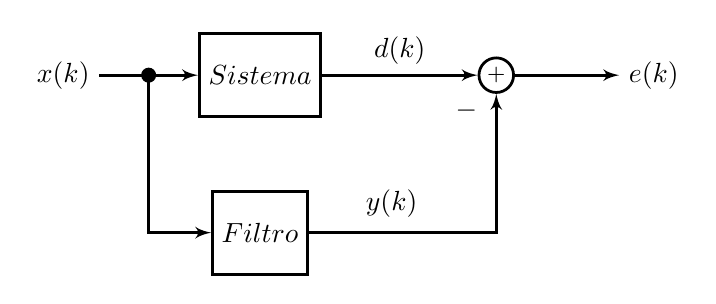
\begin{tikzpicture}[auto,>=latex']
	\tikzstyle{block} = [draw, shape=rectangle, minimum height=3em, minimum width=3em, node distance=2cm, line width=1pt]
	\tikzstyle{sum} = [draw, shape=circle, node distance=3cm, line width=1pt, minimum width=1.25em]
	\tikzstyle{branch}=[fill,shape=circle,minimum size=2pt,inner sep=0pt]
	%Creating Blocks and Connection Nodes
	\node at (-2.5,0) (input) {$x(k)$};
	\node [block] (sistema) {$Sistema$};
	\node [sum, right of=sistema, label=-120:$ - $] (sum) {};
	\node at (sum) (plus) {{\footnotesize$+$}};
	\node at (5,0) (output) {$e(k)$};
	\path (sistema) -- coordinate (med) (sum);
	\path (input) -- coordinate(branch1) (sistema);
	\node [block, below of=sistema, label={[label distance=0.6cm]3:$ y(k) $}] (filtro) {$Filtro$};
	%Conecting Blocks
	\begin{scope}[line width=1pt]
	\draw[->] (input) -- (sistema);
	\draw[->] (sistema) to node {$ d(k) $} (sum);
	\draw[->] (sum) -- (output);
	\draw[->] (branch1) node[branch] {-} |- (filtro);
	\draw[->] (filtro) -| (sum);
	\end{scope}
	\end{tikzpicture}
	\caption{Configuração utilizada no algoritmo para filtros adaptativos.}
	\label{fig:config_filtro}
\end{figure}
  \chapter{Resultados e Discussões}

\section{Resultados para $ F_0 $}
\subsection{Adaptação do filtro}

Os resultados da adaptação do filtro para uma força $F_0(t) = A_0 sin(2\pi f_0 t)$ com $ N=1000 $  e $ SNR = 90 $ são mostrados na \cref{fig:F0_1000_90_conv}. O número de coeficientes do filtro ($ N_c $) e o fator de convergência ($ \mu $) utilizados são apresentados na figura.

\begin{figure}[!h]
	\centering
	\includegraphics[scale=0.7]{F0_1000_90_conv}
	\caption{Evolução do filtro para $ F=F_0 $, $ N=1000 $ e $ SNR=90 $.}
	\label{fig:F0_1000_90_conv}
\end{figure}

Para o caso do seno puro podemos o filtro tem uma convergência rápida e com menos de 100 iterações o erro já é próximo de zero. 

Na \cref{fig:F0_1000_10_conv} são apresentados os resultados para $ N=1000 $ e $ SNR=10 $. Podemos observar que, mesmo com um nível de ruído mais elevado, o algoritmo apresentou uma convergência rápida.

\begin{figure}
	\centering
	\includegraphics[scale=0.7]{F0_1000_10_conv}
	\caption{Evolução do filtro para $ F=F_0 $, $ N=1000 $ e $ SNR=10 $.}
	\label{fig:F0_1000_10_conv}
\end{figure}

\subsection{FRF do filtro}

Na \cref{fig:F0_1000_90_FRF_med_False} é apresentada a FRF do filtro obtido com $ SNR=90 $ considerando o último vetor de coeficientes, e na \cref{fig:F0_1000_90_FRF_med_True} é apresentada a FRF considerando o vetor obtido através do valor esperado dos coeficientes tomando por base as observações da segunda metade do vetor de dados. A \cref{fig:F0_1000_10_FRF} apresenta os resultados para $ SNR=10 $. 

Podemos observar que FRF do filtro obtido não apresenta bons resultados, aproximando-se do valor esperado apenas na frequência de excitação (\SI{34}{\radian \per \s}). Podemos notar um aumento na amplitude próxima à primeira frequência natural do sistema, mas o valor não se aproxima do esperado. Outro ponto importante é que, para este caso, a FRF do filtro não se mostrou sensível ao nível de ruído. A utilização do último vetor de coeficientes $ w $ ou do valor esperado para a segunda metade do vetor de dados também não teve impacto significativo na resposta. 

\begin{figure}
	\centering
	\begin{subfigure}{0.9\textwidth}
		\centering
		\includegraphics[width=0.9\linewidth]{F0_1000_90_FRF_med_False}
		\caption{último vetor $ w $}
		\label{fig:F0_1000_90_FRF_med_False}
	\end{subfigure}
	\begin{subfigure}{0.9\textwidth}
		\centering
		\includegraphics[width=0.9\linewidth]{F0_1000_90_FRF_med_True}
		\caption{valor médio de $ w $}
		\label{fig:F0_1000_90_FRF_med_True}
	\end{subfigure}
	\caption{FRF do filtro obtido para $ F=F_0 $, $ N=1000 $ e $ SNR=90 $.}
\end{figure}

\begin{figure}
	\centering
	\begin{subfigure}{0.9\textwidth}
		\centering
		\includegraphics[width=0.9\linewidth]{F0_1000_10_FRF_med_False}
		\caption{último vetor $ w $}
		\label{fig:F0_1000_10_FRF_med_False}
	\end{subfigure}
	\begin{subfigure}{0.9\textwidth}
		\centering
		\includegraphics[width=0.9\linewidth]{F0_1000_10_FRF_med_True}
		\caption{valor médio de $ w $}
		\label{fig:F0_1000_10_FRF_med_True}
	\end{subfigure}
	\caption{FRF do filtro obtido para $ F=F_0 $, $ N=1000 $ e $ SNR=10 $.}
	\label{fig:F0_1000_10_FRF}
\end{figure}

\subsection{Predição}

Para analisarmos a predição do filtro, foi escolhida uma força arbitrária $ F_3 $ conforme \cref{eq:F_3}

\begin{equation}\label{eq:F_3}
F_3 = B_1 sin(\omega_1 t)
+ B_2 sin(\omega_2 t)
+ B_3 sin(\omega_3 t)
+ \nu
\end{equation}
onde $ B_1=\SI{1}{\N} $, $ B_2=\SI{2}{\N}$ , $ B_3=\SI{3}{\N} $, $ \omega_1= \SI{14}{\radian \per \s} $, $ \omega_2= \SI{40}{\radian \per \s} $, $ \omega_3= \SI{65}{\radian \per \s} $ e $ \nu $ é um ruído branco de variância 1.

A 

\begin{figure}[h]
	\centering
	\includegraphics[scale=0.6]{F0_1000_90_pred}
	\caption{Predição do filtro obtido com $ F=F_0 $, $ N=1000 $ e $ SNR=90 $.}
	\label{fig:F0_1000_90_pred}
\end{figure}


Assim como mostrado por \citet{castello2005experimental}, no caso analisado o fenômeno de anti-ressonância também não foi capturado pelo LMS.


  \chapter{Conclusões}

Através da construção de um filtro adaptativo para um sistema com três graus de liberdade foi possível avaliar a influência de diversos fatores no projeto do filtro.

Um filtro projetado com um sinal de entrada que possua uma frequência de excitação específica não apresenta boas predições para forçamentos diferentes daquele utilizado no processo adaptativo. Sendo assim, caso se deseje obter melhores predições para um determinado intervalo de frequência, recomenda-se que a frequência da força de entrada seja variada durante o processo de adaptação do filtro.

O ruído branco se mostrou o melhor sinal de entrada para a identificação do sistema em um determinado intervalo de frequência. O filtro construído com esse sinal de entrada e com $ SNR $ alto foi capaz de detectar os três picos referentes às frequências naturais do sistema e também o fenômeno de anti-ressonância. Além disso, o filtro foi capaz de prever com grande exatidão o comportamento do sistema para uma força diferente daquela utilizada no processo de adaptação. Para um $ SNR $ mais baixo o filtro ainda foi capaz de identificar a primeira frequência natural do sistema, mas apresentou resultados ruins para frequências afastadas do primeiro pico e também para a predição a uma força diferente da utilizada no processo de adaptação.

Com relação ao número de amostras utilizados, foi possível perceber que, para o caso de uma excitação em frequência específica, o filtro apresenta uma convergência rápida, sendo necessárias menos de 200 iterações para que o erro se aproximasse de zero. Já para o caso do ruído branco, foi necessária a utilização de um número maior de amostras e também de coeficientes para que a convergência fosse atingida.

Com relação ao fator de convergência, na seção \ref{adapt_F_1} foi possível observar como a sua escolha tem influência no processo de adaptação do filtro. No caso analisado foi possível perceber que um valor baixo diminui a velocidade de adaptação do filtro, mas um valor muito alto pode resultar na não convergência do algoritmo.


  \backmatter
  \bibliographystyle{coppe-unsrt}
  \bibliography{thesis}

  \appendix
  \chapter{Código utilizado}

Foi omitido o código utilizado para gerar o sistema utilizado (código do trabalho 1) e para plotar os gráficos apresentados no trabalho.

\begin{minted}{python3}


def F0(t):
	A0 = 1
	w0 = 33.84
	return A0*np.sin(w0*t)

def F1(t):
	A1, A2 = (1, 2)
	w1, w2 = (0.9*18, 1.1*50)
	return A1*np.sin(w1*t) + A2*np.sin(w2*t)

def F2(t):
	var = 1
	norm = stats.norm(0, np.sqrt(var))
	return norm.rvs(len(t))

def F4(t):
	A1, A2, A3 = (1, 2, 3)
	w1, w2, w3 = (0.7*20, 0.8*50, 1.3*50)
	var = 1
	norm = stats.norm(0, np.sqrt(var))
	return A1*np.sin(w1*t) + A2*np.sin(w2*t) + A3*np.sin(w3*t) + norm.rvs(len(t))
	
m0, m1, m2 = (1, 1, 1)
k0, k1, k2 = (1600, 1600, 1600)
M1 = np.array([[m0, 0, 0],
		[0, m1, 0],
		[0, 0, m2]])
K1 = np.array([[k0+k1, -k1,   0],
		[-k1, k1+k2, -k2],
		[0,     -k2,  k2]])
alpha, beta = 1e-3, 1e-3
C1 = alpha*M1 + beta*K1
sys = vt.VibSystem(M1, alpha*M1 + beta*K1, K1,
r'Sistema 1 - $\alpha = 10^{-3}$ e $\beta = 10^{-3}$')

def noise(sig, snr):
	"""
	Returns a corrupted signal based on a
	signal-to-noise ratio (SNR).
	"""
	a_s = np.sqrt((sig * sig).mean())
	a_n = a_s/10**(snr/20)
	var = a_n**2
	norm = stats.norm(0, np.sqrt(var))
	
	return sig + norm.rvs(len(sig))


class LMSFilter(object):
	def __init__(self, Nc, mu):
		"""
		Iniciar filtro com Nc coeficientes.
		"""
		self.Nc = Nc
		self.mu = mu
		# valores iniciais para o filtro w = [0, 0, ..., 0]
		self.w = np.zeros(Nc)
	
	def predict(self, x):
		y = self.w @ x
		return y
	
	def update(self, d, x):
		"""
		Atualizar filtro baseado no sinal de entrada x
		e no valor desejado d.
		"""
		y = self.w @ x
		e = d - y
		self.w += 2 * self.mu * e * x
		
class SysId(object):
	def __init__(self, name, sys, Nc, mu, F, N, snr,
	inp=2, out=0):
	self.name = name
	self.names = name.split('_')
	self.sys = sys
	self.Nc = Nc
	self.mu = mu
	self.F = F
	self.N = N
	self.snr = snr
	self.inp = inp
	self.out = out
	
	# criar filtro
	self.filt = vt.LMSFilter(Nc, mu)
	
	# criar array de tempo
	self.dt = 1/(8*(50/(2*np.pi)))
	self.t = np.linspace(0, N*self.dt, N)
	
	# criar forçamento (input)
	F_ = np.zeros((len(self.t), sys.n))
	F_[:, inp] = F(self.t)
	self.F_ = F_
	self.x = F_[:, inp]
	
	# resposta do sistema (d)
	_, _, self.sys_time_resp = sys.time_response(self.F_, self.t)
	self.d = self.sys_time_resp[:, out] # selecionar output
	
	# resposta do sistema com ruído (d_noise)
	d_n = np.copy(self.sys_time_resp.T)
	for i, sig in enumerate(d_n):
	d_n[i, :] = noise(sig, snr)
	self.sys_time_resp_noise = d_n.T
	self.d_noise = self.sys_time_resp_noise[:, out] # sel. output
	
	# atualizar filtro
	ws_hist = np.zeros((N, Nc))
	ys_hist = np.zeros(N)
	# adicionar Nc zeros ao início do input
	self.x_shift = np.concatenate([np.zeros(Nc - 1), self.x])
	for i in range(N):	
		self.filt.update(self.d_noise[i], self.x_shift[i: i + Nc])
		ys_hist[i] = self.filt.predict(self.x_shift[i: i + Nc])
		ws_hist[i] = self.filt.w

	self.w = self.filt.w
	self.ws = ws_hist
	self.ys = ys_hist
	self.e = ((self.d_noise - self.ys))
	
	def y_last_w(self, sig):
		N = self.N
		Nc = self.Nc
		sig = np.concatenate([np.zeros(Nc - 1), sig])
		y_last_w = np.zeros(N)
		for i in range(N):
		y_last_w[i] += self.filt.predict(sig[i: i + Nc])
	
	return y_last_w
	
	def freq_resp(self, sig, worN):
		fs = 1/self.dt
		w, h = signal.freqz(sig, worN=worN)
		w *= fs

	return w, h

\end{minted}

\end{document}
